\documentclass[cameraready]{Interspeech}
\usepackage{float}

\graphicspath{{../notebooks/plots/}}

% Front matter: capture abstract, then render title + abstract + TOC in one full-width block.
\makeatletter
\newbox\@abstractbox

\renewenvironment{abstract}{%
  \global\setbox\@abstractbox=\vbox\bgroup
  \hsize=\textwidth
  \small
  \setlength{\parskip}{0.45em}%
  \setlength{\parindent}{0pt}%
}{%
  \egroup
}

\renewcommand*\l@section[2]{%
  \ifnum \c@tocdepth >\z@
    \addpenalty\@secpenalty
    \addvspace{1.0em \@plus\p@}%
    \setlength\@tempdima{1.5em}%
    \begingroup
      \parindent \z@ \rightskip \@pnumwidth
      \parfillskip -\@pnumwidth
      \leavevmode \bfseries
      \advance\leftskip\@tempdima
      \hskip -\leftskip
      #1\nobreak\dotfill
      \nobreak\hb@xt@\@pnumwidth{\hss #2\kern-\p@\kern\p@}\par
    \endgroup
  \fi
}

\newcommand{\reporttableofcontents}{%
  \setcounter{tocdepth}{2}%
  \vspace{10pt}%
  \begin{center}{\bfseries\large\contentsname}\end{center}%
  \vspace{4pt}%
  \begingroup
  \small
  \@starttoc{toc}%
  \endgroup
}

\newcommand{\reportindexterms}{%
  \vspace{8pt}%
  \begingroup
  \small
  \hsize=\textwidth
  \setlength{\parindent}{0pt}%
  \setlength{\parskip}{0pt}%
  \sloppy
  \noindent\textbf{Index Terms:} \textit{\@keywords}\par
  \endgroup
}

\newcommand{\reportmaketitle}{%
  \twocolumn[{%
    \thispagestyle{empty}%
    \begin{center}%
      {\Large\bfseries \@title\par}%
      \vspace{9pt}%
      {\large\itshape \anonname\par}%
      \vspace{7pt}%
      {\normalsize \anonaddress}%
      \vspace{4pt}%
      {\small\texttt{\anonemail}}%
    \end{center}%
    \vspace{10pt}%
    \begin{center}{\bfseries\large Abstract}\end{center}%
    \vspace{5pt}%
    \unvbox\@abstractbox
    \reportindexterms
    \vspace{6pt}%
    \reporttableofcontents
    \vspace{4pt}%
  }]%
}
\makeatother

\title{Generative Models for Cat Face Synthesis: \\ A Comparative Study of Variational Autoencoders, Generative Adversarial Networks, and Diffusion Models}

\author[affiliation={1}]{Pawel}{Pozorski}
\author[affiliation={1}]{Pawel}{Florek}

\address{
    $^1$ Warsaw University of Technology, Poland
}

\email{\{pawel.pozorski, pawel.florek\}.stud@pw.edu.pl}

\keywords{generative models, variational autoencoders, generative adversarial networks, diffusion models, PixelCNN, latent diffusion, image synthesis, cat generation, FID, hyperparameter optimization, mode collapse}

\begin{document}

\begin{abstract}
This report presents a comparative study of three major generative modeling paradigms---Variational Autoencoders (VAE), Generative Adversarial Networks (GAN), and Diffusion Models---applied to the synthesis of $128 \times 128$ cat face images. We evaluate $\beta$-VAE and VQ-VAE-1 (VAE family), WGAN-GP and SN-GAN (GAN family), DDIM and a Tiny Latent Diffusion Model (diffusion family), and add a classical PixelCNN autoregressive prior over VQ-VAE code indices as a baseline for latent generative modeling. The study employs structured grid search over key hyperparameters. We evaluate models using Fréchet Inception Distance (FID), latent interpolations, and a qualitative comparison of PixelCNN versus Tiny LDM (sample quality and wall-clock generation time). Furthermore, we conduct an exploratory \emph{chimera} extension: WGAN-GP trained on $\sim 25{,}000$ mixed dogs-and-cats images at $64 \times 64$ to observe distribution averaging phenomena. This work provides a practical framework for comparing generative paradigms.
\end{abstract}

\reportmaketitle

\clearpage
\section{Introduction}

Generative modeling of images has been a central research challenge in machine learning, with three primary paradigms emerging over the past decade: Variational Autoencoders (VAEs) \cite{kingma2013auto}, Generative Adversarial Networks (GANs) \cite{NIPS2014_f033ed80}, and Diffusion Models \cite{NEURIPS2020_4c5bcfec}. Each paradigm offers distinct theoretical foundations, training dynamics, and trade-offs in quality, diversity, and training stability. VAEs provide a principled probabilistic framework but often produce blurrier samples; GANs generate sharp images but suffer from training instability and mode collapse; diffusion models have recently demonstrated superior sample quality but require longer inference times.

The selection of appropriate generative models for practical applications remains highly dependent on specific constraints: available computational resources, target sample quality, required inference speed, and stability during training. In this project, we conduct a systematic comparison of representative architectures across all three paradigms on a well-defined task: generating cat face images from the Kaggle Cat Dataset.

Our objectives align with the specific project requirements: (i) standardize varying image resolutions utilizing raw annotation data to accommodate limited computing resources; (ii) systematically compare generation quality across three paradigms (VAE, GAN, Diffusion) using quantitative metrics (FID) and qualitative assessment; (iii) directly address mode collapse through stabilized GAN architectures (WGAN-GP with gradient penalty, SN-GAN with spectral normalization); (iv) analyze latent space smoothness via interpolation: generating 10-image sequences (2 random endpoints + 8 linear intermediates) to assess semantic continuity; and (v) explore cross-species generalization via a \emph{chimera} experiment: WGAN-GP on mixed ``Dogs vs. Cats'' data at $64 \times 64$ to investigate whether the unconditional model learns to separate classes or exhibits distribution averaging (e.g., chimera-like outputs).

\section{Methodology}

\subsection{Datasets and Preprocessing}

The primary dataset consists of over 9,000 cat images sourced from the Kaggle Cat Dataset \cite{crawford2018cat}. Raw images exhibit significant variability in resolution, aspect ratio, and face positioning, which poses a challenge for batch processing and limited computing resources. To address this, we apply the following preprocessing pipeline:

\begin{enumerate}
    \item \textbf{Annotation Parsing}: Instead of relying on pre-trained face detectors, we extract the exact 9 coordinate points (eyes, mouth, ears) provided in the corresponding \texttt{.cat} annotation files.
    \item \textbf{Face Cropping}: Bounding boxes are dynamically calculated based on the extreme coordinates of the facial landmarks with a $35\%$ pad on the landmark extent (\texttt{BBOX\_PAD\_RATIO}$=0.35$).
    \item \textbf{Resizing}: Cropped regions are standardized to $128 \times 128$ pixels using Lanczos resampling (\texttt{PIL.Image.LANCZOS}), drastically reducing VRAM footprint and training time.
    \item \textbf{Normalization}: All cat-face training tensors are mapped to $[-1, 1]$ via \texttt{ToTensor} and per-channel normalization with mean $0.5$ and std $0.5$, matching $\tanh$ decoder/generator outputs; pixel DDIM sampling clamps predicted images to $[-1, 1]$ each step.
    \item \textbf{Training augmentation}: The cat-face train split applies \texttt{RandomHorizontalFlip} ($p{=}0.5$); validation tensors are not augmented.
\end{enumerate}

Processed images are written to \texttt{train.npy} and \texttt{val.npy} using a $90/10$ train/validation split with a fixed assignment seed ($42$).

Comparison of raw vs. processed images is shown in Figure~\ref{fig:preprocessing_comparison}.

\begin{figure}[H]
    \centering
    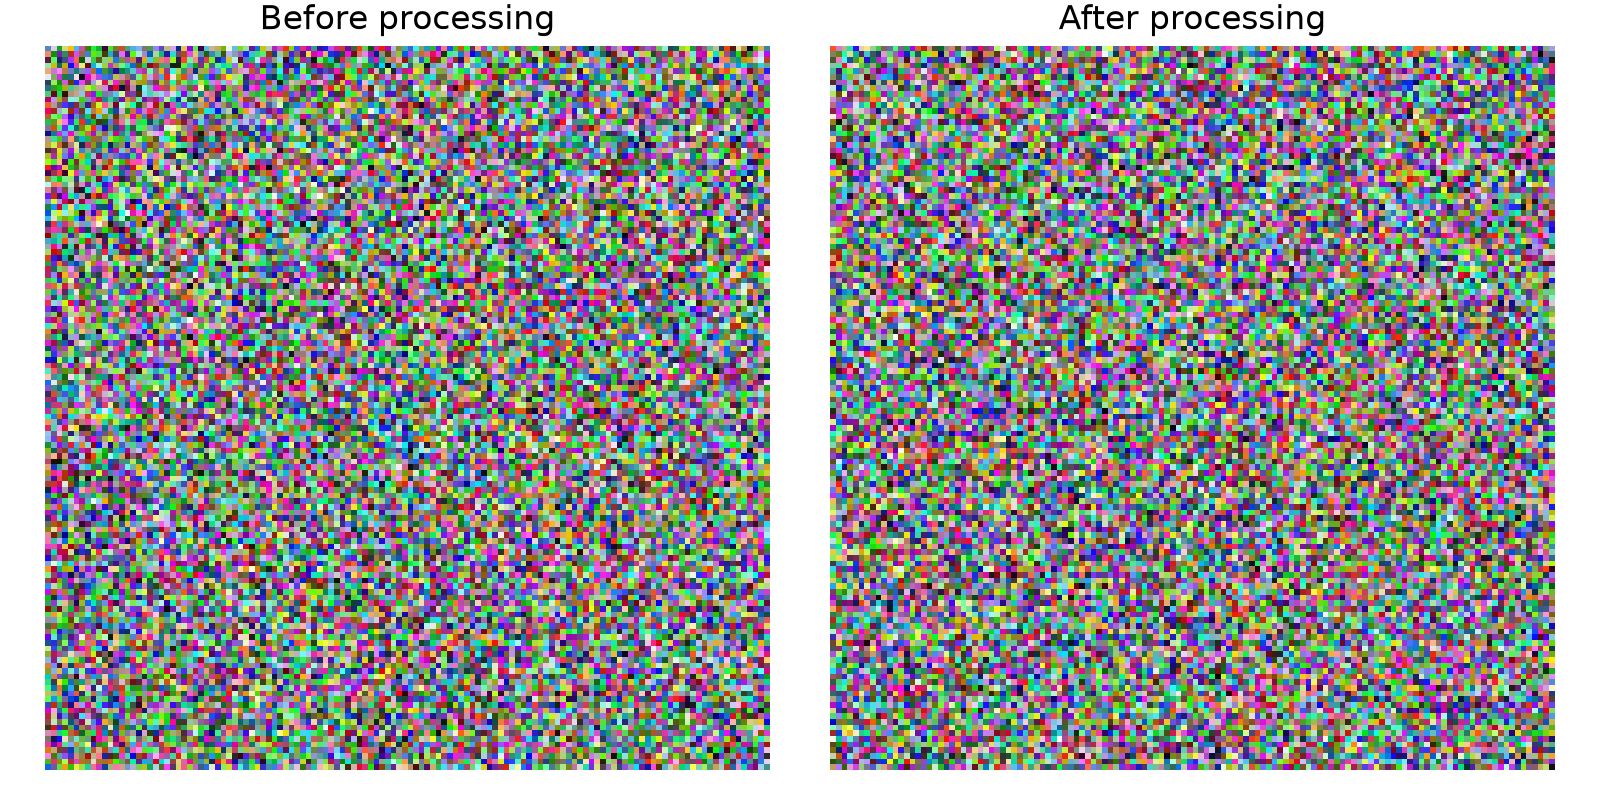
\includegraphics[width=\linewidth]{preprocessing_comparison.png}
    \caption{Sample images after preprocessing: cropped and resized to $128 \times 128$ pixels.}
    \label{fig:preprocessing_comparison}
\end{figure}

For the exploratory chimera extension, we utilize the Kaggle "Dogs vs. Cats" competition benchmark dataset \cite{dogs-vs-cats}, which contains $\sim 25{,}000$ mixed images (Figure~\ref{fig:mixed_samples}). Since this dataset lacks facial landmark annotations, applying the coordinate-based cropping procedure is impossible. Instead, we apply the same scale-and-crop strategy at $64 \times 64$: resize the shorter edge to 64 pixels, then extract a $64 \times 64$ center crop, and store the result as \texttt{dogcat\_train\_64.npy} for training.

\begin{figure}[H]
    \centering
    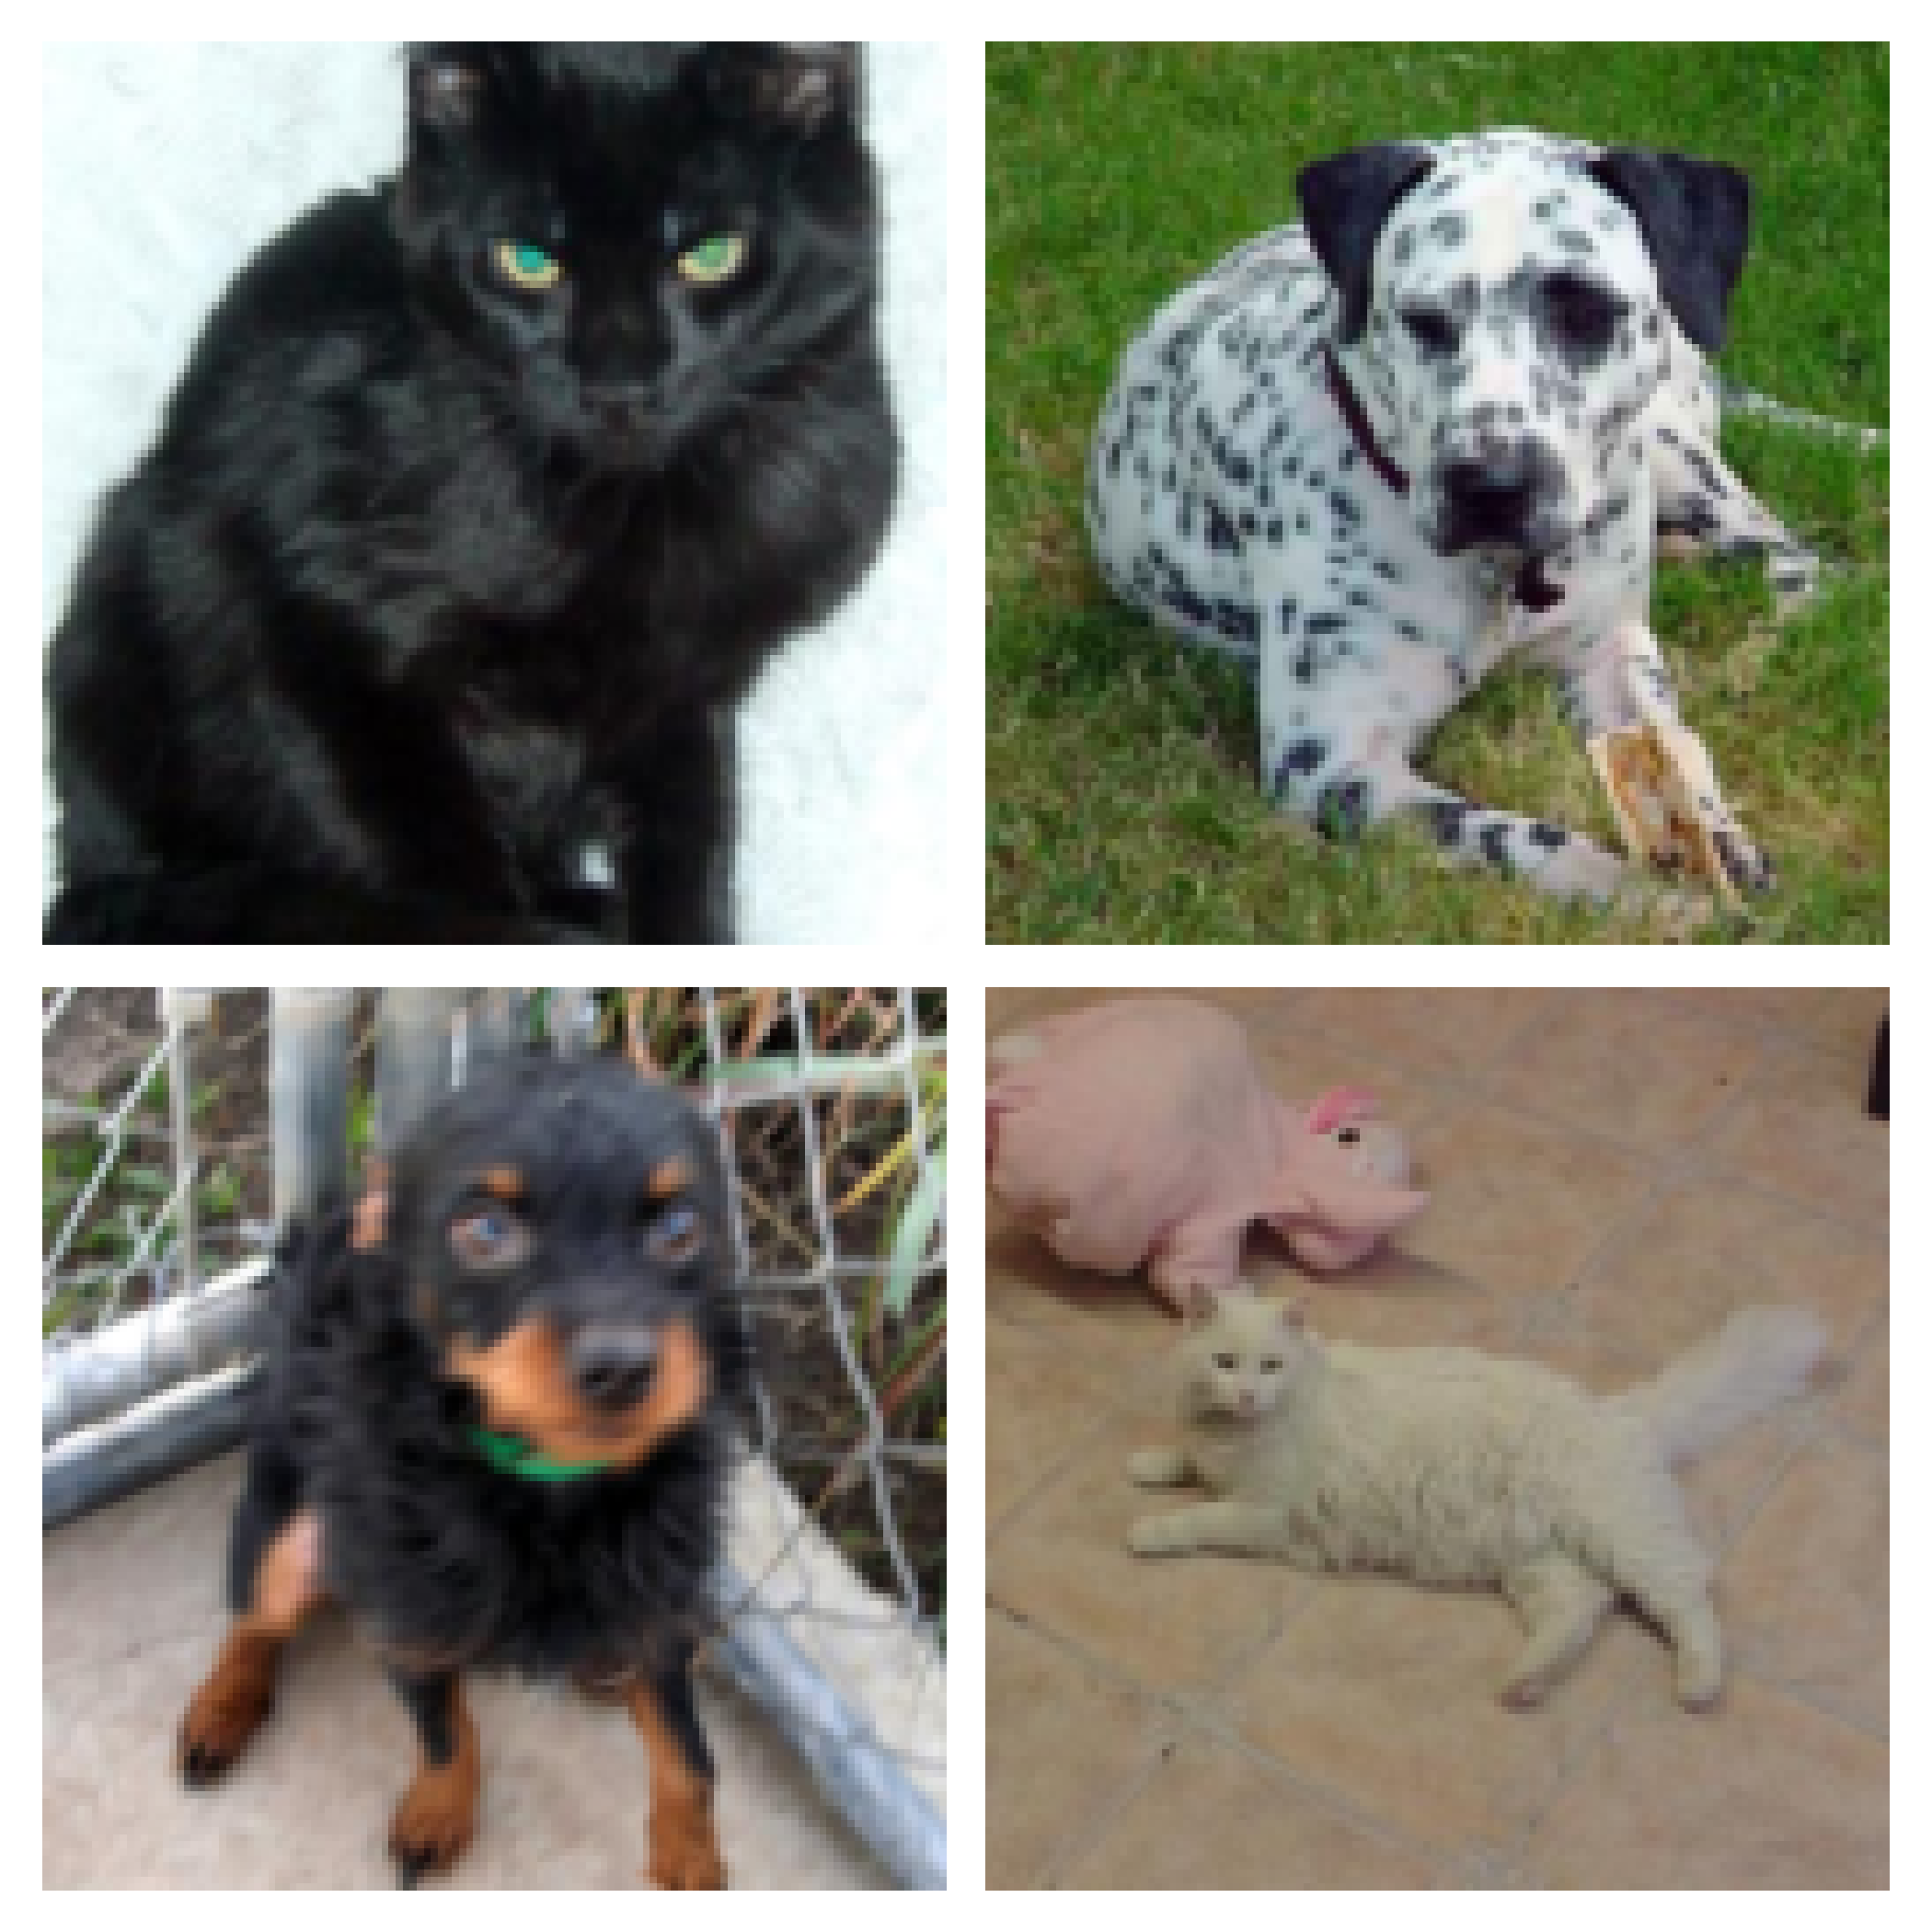
\includegraphics[width=\linewidth]{processed_samples_dogcat.png}
    \caption{Sample images from the mixed "Dogs vs. Cats" dataset after scale-and-crop preprocessing (chimera pipeline uses $64 \times 64$ tensors).}
    \label{fig:mixed_samples}
\end{figure}

\subsection{Generative Model Architectures}

\begin{description}[leftmargin=1.25em, labelsep=0.5em, itemsep=0.6em, topsep=0.4em]
\item[Variational Autoencoders (VAE)]
VAEs define a probabilistic generative model via a learned latent variable distribution $q_\phi(z|x)$ parameterized by an encoder network. The generative process is specified by a decoder $p_\theta(x|z)$ where $z \sim \mathcal{N}(0, I)$. We evaluate two VAE variants:

\textbf{$\beta$-VAE \cite{higgins2017betavae}:} A standard VAE with convolutional encoder/decoder and a $\beta$ parameter that controls the trade-off between reconstruction accuracy and prior matching. Grid search varies: $\text{latent\_dim} \in \{64, 128\}$, $\beta \in \{1.0, 4.0\}$.

\textbf{VQ-VAE-1:} A discrete VAE using vector quantization in the latent space \cite{NIPS2017_7a98af17}. Instead of a continuous distribution, VQ-VAE discretizes the latent space into a learned codebook to reduce the blurriness typical of standard VAEs. Grid search varies: $\text{codebook\_size} \in \{512, 1024\}$, $\text{feat\_map\_size} \in \{16 \times 16, 8 \times 8\}$, and reconstruction loss (L1 vs.\ MSE). Non-swept defaults are $\text{embedding\_dim}=64$ and $\text{commitment\_cost}=0.25$.

\item[Generative Adversarial Networks (GAN)]
GANs formulate image generation as an adversarial game between a generator $G$ and discriminator $D$. To directly address the mode collapse problem required by this study, we avoid the standard DCGAN and evaluate two stabilized variants:

\textbf{WGAN-GP:} Wasserstein GAN \cite{pmlr-v70-arjovsky17a} with gradient penalty \cite{NIPS2017_892c3b1c} uses the Wasserstein distance and adds a gradient penalty term to enforce the Lipschitz constraint, significantly reducing mode collapse and providing meaningful learning curves. Both GAN generators use a fixed latent dimension of $128$. Grid search varies: $\text{n\_critic} \in \{3, 5\}$, batch size $\in \{64, 128\}$, learning rate schedule $\in \{\text{symmetric}, \text{TTUR}\}$.

\textbf{SN-GAN:} Spectral Normalization GAN \cite{DBLP:journals/corr/abs-1802-05957} stabilizes discriminator training by normalizing weights with their largest singular value. Training uses one discriminator update per generator step and hinge losses. Grid search varies: batch size $\in \{64, 128\}$, learning rate schedule $\in \{\text{symmetric}, \text{TTUR}\}$, horizontal flip augmentation.

\item[Diffusion Models]
Diffusion models define a forward process that corrupts images to noise, then learn to reverse this process via a neural network. To mitigate the immense computational cost of diffusion, we focus on optimized architectures:

\textbf{DDIM:} A faster sampling approach for diffusion models \cite{DBLP:journals/corr/abs-2010-02502} that uses a deterministic sampling procedure, enabling inference in fewer steps. A U-Net denoises $128 \times 128$ pixel images with an $8 \times 8$ bottleneck over $T{=}1000$ forward diffusion steps; an exponential moving average (EMA) copy of the U-Net is used for validation and sampling. Grid search varies: noise schedule $\in \{\text{linear}, \text{cosine}\}$, base channels $\in \{64, 128\}$, and DDIM steps $\in \{50, 100\}$ (stored in each checkpoint and used at generation time).

\textbf{Tiny Latent Diffusion Model (LDM):} Following Rombach et al. \cite{Rombach_2022_CVPR}, we train a lightweight U-Net diffusion model on \emph{continuous} pre-quantization latents from a frozen VQ-VAE-1 encoder; vector quantization is applied only at decode time. Latent activations are scaled to unit variance using validation-set statistics before diffusion training. The VQ encoder/decoder weights are not updated during LDM training; only the U-Net (and its EMA copy) is optimized. DDIM sampling produces a latent tensor that is unscaled, quantized, and passed through the frozen decoder. The frozen VQ-VAE per seed is chosen from the VQ grid sweep as the checkpoint with lowest validation reconstruction loss (\texttt{prior\_best\_by\_seed.json}). Grid search matches DDIM: schedule $\in \{\text{linear}, \text{cosine}\}$, base channels $\in \{64, 128\}$, DDIM steps $\in \{50, 100\}$.

\item[PixelCNN Prior over VQ Codes (Baseline)]
VQ-VAE-1 alone defines $p(x|z)$ via the decoder but not a prior $p(z)$ over discrete code indices. For unconditional synthesis we therefore compare two learned priors on the same frozen VQ-VAE:

\textbf{PixelCNN \cite{oord2016pixel}:} A lightweight autoregressive model with masked convolutions predicts codebook indices on the $16 \times 16$ or $8 \times 8$ latent grid (depending on the VQ-VAE configuration). Architecture is fixed at 128 hidden channels and 10 masked layers (not swept). After the VQ-VAE grid sweep, PixelCNN is trained once per seed on the manifest-selected frozen VQ-VAE; a follow-up \texttt{pixelcnn-experiment} script also trains a single Tiny LDM configuration per seed (EMA on, DDIM steps $=100$) for wall-clock and qualitative comparison against PixelCNN.
\end{description}

\subsection{Training Setup and Hyperparameter Grid}

All models employ the Adam optimizer \cite{kingma2014adam} with $\text{lr} = 2 \times 10^{-4}$ and $(\beta_1, \beta_2) = (0.5, 0.999)$ for VAE, diffusion, and PixelCNN trainers. GAN generators use $(\beta_1, \beta_2) = (0.5, 0.999)$ under WGAN-GP and $(0.0, 0.9)$ under SN-GAN. Training uses a high epoch cap ($1000$) with early stopping (patience $= 15$, $\text{min\_epochs} = 20$, $\text{min\_delta} = 10^{-4}$). $\beta$-VAE and VQ-VAE early stopping monitor \textbf{reconstruction loss} rather than total loss (which includes KL or VQ terms that can plateau early). PixelCNN and diffusion trainers monitor validation loss; GAN early stopping monitors generator loss (\texttt{g\_loss}). SN-GAN horizontal-flip augmentation applies only to real images fed to the discriminator when enabled in the grid. All main experiments use Apple MPS unless overridden; metrics and sample grids are logged to MLflow.

Symmetric vs.\ TTUR learning-rate schedules \cite{heusel2017gans} are implemented by pairing generator learning rate $2 \times 10^{-4}$ with discriminator learning rate $\in \{2 \times 10^{-4}, 4 \times 10^{-4}\}$.

Each hyperparameter configuration is trained independently across three fixed random seeds $\{42, 0, 3407\}$. Seeds are reset in PyTorch, NumPy, and Python before every run. Grid-sweep results are compared per cell; evaluation metrics are aggregated over the same seed list for reproducibility. Table~\ref{tab:hyperparam_grid} lists the search space per family; the \textbf{Runs} column counts trained jobs as (grid cells) $\times$ 3 seeds. The main cat-face protocol comprises $135$ such runs. The \texttt{pixelcnn-experiment} pipeline adds three fixed-configuration Tiny LDM trainings (DDIM steps $=100$, EMA on) for prior wall-clock comparison against PixelCNN. The chimera extension adds three further WGAN-GP runs at $64 \times 64$ ($141$ training jobs in total).


\begin{table}[H]
    \centering
    \caption{Hyperparameter grid summary across generative model families.}
    \label{tab:hyperparam_grid}
    \renewcommand{\arraystretch}{1.4}
    \resizebox{\linewidth}{!}{%
    \begin{tabular}{|l|l|l|r|}
        \hline
        \textbf{Model Family} & \textbf{Parameter} & \textbf{Search Space} & \textbf{Runs} \\
        \hline
        $\beta$-VAE & latent\_dim, $\beta$ & $\{64, 128\} \times \{1.0, 4.0\}$ & 12 \\
        VQ-VAE-1 & codebook, map, loss & $\{512, 1024\} \times \{16, 8\} \times \{L1, MSE\}$ & 24 \\
        WGAN-GP & n\_critic, batch, LR & $\{3, 5\} \times \{64, 128\} \times \{sym, TTUR\}$ & 24 \\
        SN-GAN & batch, LR, augment & $\{64, 128\} \times \{sym, TTUR\} \times \{no, hflip\}$ & 24 \\
        DDIM & schedule, ch., steps, EMA & $\{lin., cos.\} \times \{64, 128\} \times \{50, 100\}$, EMA on & 24 \\
        Tiny LDM & schedule, ch., steps, EMA & same as DDIM (frozen VQ latents) & 24 \\
        PixelCNN prior & hidden width, depth & $128$ channels, $10$ masked layers (fixed) & 3 \\
        \hline
        \multicolumn{3}{|r|}{\textbf{Total (cat-face sweeps)}} & \textbf{135} \\
        \hline
    \end{tabular}%
    }
    \vspace{4pt}
    {\small Includes $135$ cat-face grid jobs; add $+3$ fixed Tiny LDM prior runs and $+3$ chimera jobs for $141$ trainings total (see text).}
\end{table}

\subsection{Evaluation Metrics}

\begin{description}[leftmargin=1.25em, labelsep=0.5em, itemsep=0.6em, topsep=0.4em]
\item[Fréchet Inception Distance (FID)]
FID \cite{heusel2017gans} compares the distribution of real validation images to unconditionally generated samples in the feature space of a pretrained Inception-v3 network. Lower FID indicates better alignment with the data distribution. We use each model's native sampling procedure (e.g., $z \sim \mathcal{N}(0,I)$ for $\beta$-VAE and GANs, DDIM for pixel diffusion, random codes for VQ-VAE when no separate prior is evaluated). Generated tensors in $[-1,1]$ are denormalized to $[0,1]$, resized to $299 \times 299$, and passed through Inception-v3 with ImageNet input normalization before feature extraction.

We report FID on the held-out validation set for every trained family: $\beta$-VAE, VQ-VAE-1, PixelCNN, Tiny LDM, WGAN-GP, SN-GAN, and DDIM, using a fixed sample count ($N{=}1000$) per run. For each model family we evaluate \textbf{every} hyperparameter grid cell that has a \texttt{best} checkpoint: FID is computed independently per seed, then mean $\pm$ standard deviation is reported per cell; the cell with the lowest mean FID is recorded as \texttt{best\_run}. For VQ-linked models (VQ-VAE, PixelCNN, Tiny LDM), frozen VQ weights per seed come from \texttt{prior\_best\_by\_seed.json} (lowest validation reconstruction across the VQ sweep). PixelCNN and Tiny LDM use their learned priors with that frozen decoder; VQ-VAE FID uses the trainer's random-code debug sampler and is reported only as a weak baseline, not comparable to the learned priors.

\item[Latent Interpolation Analysis]
For models with a continuous latent vector $z \in \mathbb{R}^d$, we test whether the learned representation is semantically smooth. We sample two endpoints $z_1, z_2 \sim \mathcal{N}(0,I)$ from the prior used at generation time, form eight uniformly spaced convex combinations
$z_\alpha = (1-\alpha) z_1 + \alpha z_2$, $\alpha \in \{0, \tfrac{1}{9}, \ldots, 1\}$,
and decode each $z_\alpha$ to an image, yielding a strip of ten frames. Continuity of appearance along the strip is judged qualitatively. This protocol is applied to $\beta$-VAE and WGAN-GP using the \texttt{best\_run} hyperparameter cell from \texttt{fid\_scores.json} (lowest mean FID); it is not used for discrete VQ codes or diffusion latents without an explicit interpolation definition.

\item[PixelCNN vs.\ Tiny LDM Prior Comparison]
Using the same frozen VQ-VAE per seed, we compare autoregressive PixelCNN sampling against Tiny LDM (DDIM steps $=100$, EMA) on wall-clock generation time and side-by-side sample grids. Timings use device synchronization on Apple MPS; outputs are written to \texttt{results/prior\_comparison/}.

\item[Exploratory Extension: Mixed Distributions (Chimera)]
We train WGAN-GP on a mixed dataset containing both cats and dogs at $64 \times 64$ resolution ($\sim 25{,}000$ combined images, 90/10 train/val split per seed). The goal is to observe whether the unconditional model learns to separate the classes into mode-specific outputs or suffers from distribution averaging, resulting in generating ``chimeras'' (e.g., cat faces with dog ears or dog faces with feline features). This experiment probes the limits of unconditional generation under multi-modal input distributions. WGAN-GP was chosen as a stabilized adversarial baseline at reduced resolution for compute efficiency on the full mixed dataset. Diffusion models were too computationally expensive for $\sim 25{,}000$ images, and VAEs were rejected because blurred reconstructions would obscure distribution averaging. Training uses the same early-stopping hyperparameters as the main cat study but defaults to a lower epoch cap ($100$) for this exploratory run; all three project seeds $\{42, 0, 3407\}$ are trained independently.
\end{description}

\section{Results}

\subsection{Fr\'echet Inception Distance}
[To be populated from \texttt{results/fid\_scores.json}.]

\subsection{Qualitative Samples}
[To be populated from \texttt{make additional-samples} and training checkpoints.]

\subsection{Latent Interpolation}
[To be populated from \texttt{results/interpolations/}.]

\subsection{PixelCNN vs.\ Tiny LDM}
[To be populated from \texttt{results/prior\_comparison/}.]

\subsection{Chimera Extension}
[To be populated from \texttt{checkpoints/chimera/}.]

\section{Conclusions}
[To be populated]

\section{AI Disclosure}

This report was edited with AI assistance, to improve clarity, consistency, and formatting. Part of the docstrings, some phrasing and code refactoring or debugging were refined using AI tools, but all scientific decisions and interpretations are the authors' own. The core content, experimental design, and analysis were developed by the authors.

\bibliographystyle{IEEEtran}
\bibliography{mybib}

\appendix

\section{Additional Experimental Details}
\textbf{End-to-end protocol.} \texttt{make setup} $\rightarrow$ download/process cat data $\rightarrow$ \texttt{make run-all} (VAE, GAN, diffusion sweeps; VQ prior manifest; PixelCNN experiment) $\rightarrow$ \texttt{make eval} (FID + interpolations) $\rightarrow$ optional \texttt{make chimera} after \texttt{make process-dogcat-chimera}. Regenerate report figures with \texttt{make report-figures} after \texttt{make process-data}.

\textbf{Pipeline order.} \texttt{make run-all} executes VAE, GAN, and diffusion grid sweeps, writes the VQ-VAE prior manifest, then runs the PixelCNN experiment (train PixelCNN $\times$3 seeds, train one Tiny LDM config per seed for prior comparison, wall-clock sample grids).

\textbf{Logging.} MLflow records hyperparameters, train/validation metrics, periodic $4 \times 4$ sample grids, and \texttt{samples\_best.png} from the best checkpoint. Finished runs are not resumed on restart.

\textbf{Prior comparison.} PixelCNN vs.\ Tiny LDM generation time is measured with device synchronization on Apple MPS; outputs land in \texttt{results/prior\_comparison/}.

\textbf{Checkpoints.} Best weights are saved per run as \texttt{best\_seed\{seed\}.pt} inside \texttt{checkpoints/<model\_type>/<slug>/}. Chimera training uses \texttt{checkpoints/chimera/}.

\section{Code Availability}
All code, configurations, and training logs are available at: \url{https://github.com/FlorekPawel/gen-cats}

\end{document}
